\section{Профиль и протокол}

\subsection{Цель и теоретические сведения}
Цель работы --- выяснить, как инициализация и остаточные связи влияют на сохранение сигнала, градиенты и обучение глубоких сетей, а затем проверить основной вывод на трёх seed. Протокол и критерии взяты из методических указаний~\cite{teacher}.

Номера вида (1.x) в анализе относятся к формулам исходного задания; основные используемые зависимости приведены ниже.

Для слоя $h_l=\phi(N_l(W_lh_{l-1}+b_l))$ измеряется средний квадрат $q_l=\mathbb E[h_l^2]$. При независимых центрированных весах, нулевых смещениях и ReLU приближение имеет вид
\begin{equation}q_l=\chi_lq_{l-1},\qquad\chi_l=n_{l-1}\sigma_l^2/2.\end{equation}
Поэтому He даёт $\chi=1$, Xavier при равной ширине --- $1/2$, а фиксированное $\sigma=0.02$ при $n=256$ --- $0.0512$. Небольшое отклонение от единицы накапливается с глубиной. Для BatchNorm статистики вычисляются по batch, для LayerNorm --- по признакам отдельного объекта; обязательные серии ниже выполняются без этих нормализаций.

Остаточный блок $h_{l+1}=h_l+\alpha F_l(h_l)$ имеет якобиан $I+\alpha\partial F_l/\partial h_l$. При общем коэффициенте ветви $c$ ожидается
\begin{equation}q_L/q_0\approx(1+\alpha^2c)^L.\end{equation}
Масштаб $\alpha=L^{-1/2}$ ограничивает это приближение величиной $e^c$; прямой путь при $\alpha=1$ сам по себе не ограничивает рост сигнала.

Измеряемые показатели обучаемости определены как
\begin{equation}\rho_T=\frac{\mathcal L_T}{\ln10},\quad
g_l=\frac{\|\nabla_{\theta_l}\mathcal L\|_2}{\sqrt{|\theta_l|}},\quad
GI=\log_{10}\frac{\max_l\widetilde g_l+\varepsilon}{\min_l\widetilde g_l+\varepsilon},\end{equation}
\begin{equation}AVD=\max_l|\log_{10}(v_l+\varepsilon)-\log_{10}(v_1+\varepsilon)|.\end{equation}
Здесь $\mathcal L_T$ --- cross-entropy на фиксированной обучающей подвыборке, $\widetilde g_l$ --- медиана по измеряемым шагам, $v_l$ --- дисперсия активаций, $\varepsilon=10^{-12}$. Значения $\rho_T\le0.5$ и $\rho_T\ge0.9$ задают обучаемый и необучаемый режимы; остальные значения пограничны.

\subsection{Фактический протокол}

Глубины 8, 24, 48, 96; ширина 256; $\sigma=0.02$; SGD с импульсом 0.9. Использован CIFAR-10, допустимый по §6 задания. Данные и единый цикл обучения унаследованы из ЛР0.


Полная обучающая роль: 43000 изображений; val 5000; cal 2000; test 10000. Выбор условий не использует test. Нормализация вычислена только по train. В ЛР1 используется вся обучающая роль, а не 25\%, использованные в ЛР0.

Использовано стратифицированное разбиение ЛР0 с seed 1729: по 500 объектов каждого класса для val и по 200 для cal. Роль cal не используется.

Три полные эпохи; batch 128; weight decay 0; постоянная скорость обучения; без AMP и ограничения градиента. Для завершённых трёхэпоховых обучений сохранены 1008 шагов; для одноэпоховой проверки Gaussian -- 336. Численные сбои остановлены раньше и зарегистрированы отдельно. Архитектура, seed, хеши кода/данных и точный RUN\_ID находятся в паспорте. Обозначения Rxx ниже разрешаются в полные RUN\_ID в реестре в конце отчёта.

Обычная сеть имеет $L$ скрытых линейных слоёв. Остаточная сеть содержит входную проекцию 3072$\to$256 и $L$ блоков, по два линейных слоя в каждом; после сложения нет активации. Поэтому число параметров и линейных преобразований различается; сравнение архитектур не является сравнением равных бюджетов параметров.

Проба: первые 64 фиксированных объекта train, режим eval, $\|u\|=1$, генератор $u$ из seed профиля 987693601. Для измерений используется float64-копия исходных float32-весов. Это исключает потерю очень малых сигналов при диагностике; обучение остаётся float32. Копирование не меняет веса, режим, BN-буферы, RNG и градиенты обучаемой модели.

Окончательная $\rho_T=L_T/\ln10$ измеряется по первым 1024 фиксированным объектам train после обучения. GI вычисляется по всем непосредственно параметризованным слоям, включая проекцию и классификатор: сначала медиана $g_l=\|\nabla_{\theta_l}L\|/\sqrt{|\theta_l|}$ по первому, среднему и последнему batch каждой эпохи, затем $\log_{10}[(\max g_l+10^{-12})/(\min g_l+10^{-12})]$. Вес и bias входят в один слой. AVD вычисляется по дисперсиям скрытых выходов фиксированной eval-пробы, включая $h_0$ остаточной сети. Максимальная доля нулей берётся на настоящих ReLU-выходах, а не на сумме ветви и skip.

Монитор также сохраняет среднее, std, min/max, второй момент, насыщение tanh при $|1-h^2|<0.1$, нормы и относительные нормы градиента. Квадраты вычисляются после приведения к float64. Отсутствующий градиент классификатора в линейной пробе отмечен как unused, а не как нулевой измеренный градиент.


Скорость обучения выбрана один раз по максимальной итоговой val accuracy; при равенстве используется меньшая val loss, затем меньшая LR. Все кандидаты обучались три эпохи. Выбрана LR=0.003.



\begin{table}[H]\centering\small\setlength{\tabcolsep}{4pt}
\caption{Выбор единой скорости обучения по validation, три эпохи.}
\FitTable{\begin{tabular}{lrrr}
\toprule
LR & val accuracy & val loss & Источник \\
\midrule
0.001 & 0.4298 & 1.589 & R17 \\
0.003 & 0.4558 & 1.51 & R18 \\
0.01 & 0.4558 & 1.52 & R19 \\
0.03 & 0.4498 & 1.561 & R20 \\
0.1 & 0.37 & 1.717 & R21 \\
\bottomrule
\end{tabular}}
\end{table}



\section{E1: сигнал и градиент при инициализации}

Заранее записанная гипотеза: по (1.4)--(1.8) ожидаются $\chi=1$ (He), $0.5$ (Xavier), $n\sigma^2/2=0.0512$ (Gaussian). Выполнены все 12 комбинаций без оптимизатора. Множители оцениваются геометрически между равными по ширине скрытыми слоями; при $q<10^{-30}$ применяется правило исключения из PDF. Для Gaussian L=96 эффективная конечная точка может быть раньше последнего слоя; это не замена полного обратного прохода.

\begin{table}[H]\centering\small\setlength{\tabcolsep}{4pt}
\caption{Предсказанный и измеренные множители при инициализации.}
\FitTable{\begin{tabular}{lrrrrrr}
\toprule
Init & L & $\chi$ & $\hat\chi_f$ & $\hat\chi_b$ & $L_{eff}$ & Источник \\
\midrule
he & 8 & 1 & 1.004 & 0.9898 & 8 & R05 \\
he & 24 & 1 & 1.015 & 1.012 & 24 & R06 \\
he & 48 & 1 & 0.9772 & 1.009 & 48 & R07 \\
he & 96 & 1 & 0.9804 & 0.9947 & 96 & R08 \\
xavier & 8 & 0.5 & 0.5018 & 0.4949 & 8 & R09 \\
xavier & 24 & 0.5 & 0.5076 & 0.5062 & 24 & R10 \\
xavier & 48 & 0.5 & 0.4886 & 0.5045 & 48 & R11 \\
xavier & 96 & 0.5 & 0.4902 & 0.4973 & 96 & R12 \\
gaussian & 8 & 0.0512 & 0.05138 & 0.05068 & 8 & R13 \\
gaussian & 24 & 0.0512 & 0.05198 & 0.05183 & 24 & R14 \\
gaussian & 48 & 0.0512 & 0.05221 & 0.05065 & 24 & R15 \\
gaussian & 96 & 0.0512 & 0.0499 & 0.05042 & 23 & R16 \\
\bottomrule
\end{tabular}}
\end{table}

На максимальной глубине относительные ошибки (forward; backward): he: 1.964\%; 0.533\%; xavier: 1.964\%; 0.533\%; gaussian: 2.536\%; 1.521\%. Все шесть сравнений проверяются с допуском 20\%.

Граница применимости: Gaussian после одной полной эпохи с выбранной общей LR. Результаты повторной пробы:

\begin{table}[H]\centering\small\setlength{\tabcolsep}{4pt}
\caption{Повторная проба Gaussian после одной эпохи обучения.}
\FitTable{\begin{tabular}{lrrrrr}
\toprule
L & $\hat\chi_f$ & $\hat\chi_b$ & Учтено / посл. слой & $\rho_T$ & Источник \\
\midrule
8 & 0.09712 & 0.04066 & 8 / 8 & 1 & R34 \\
24 & 0.4029 & 0.02549 & 24 / 24 & 1 & R35 \\
48 & 0.5668 & -- & 39 / 47 & 1 & R36 \\
96 & 0.0499 & 0.05042 & 23 / 23 & 1 & R37 \\
\bottomrule
\end{tabular}}
\end{table}

Прочерк в backward для R36 означает неопределённую оценку: q последнего скрытого выхода=0, средний квадрат delta первого слоя=0. Последний ReLU равен нулю на всей фиксированной пробе, и все предыдущие delta равны нулю. Отношение 0/0 не заменяется нулём или теоретическим множителем. Все эти значения конечны; флаг NaN/Inf поэтому не ставится.

Для R37 максимальная медиана g скрытых слоёв при реальном float32-обучении равна 0. Ненулевой градиент float64-пробы не означает ненулевого градиента при float32-обучении: численное обнуление путей и статистика в повышенной точности должны различаться.

Уже первое обновление SGD связывает веса с обучающими входами через градиент и в общем случае меняет нулевые bias. Поэтому исходные независимые случайные веса и нулевые смещения (1.4) больше не предполагаются. Эти нарушения возникают в одном шаге оптимизатора; измерение после эпохи не позволяет приписать одному из них более ранний момент. Совпадение части множителей с теорией не восстанавливает предположения; изменение bias способно создать сигнал даже при затухающих весовых путях.

Проверка фактических checkpoint: максимальное абсолютное bias после эпохи R34: 0.005028; R35: 0.005018; R36: 0.005015; R37: 0.005017. Начальное bias во всех случаях равно нулю; агрегат включает классификатор и скрытые слои.

\clearpage

\begin{figure}[H]\centering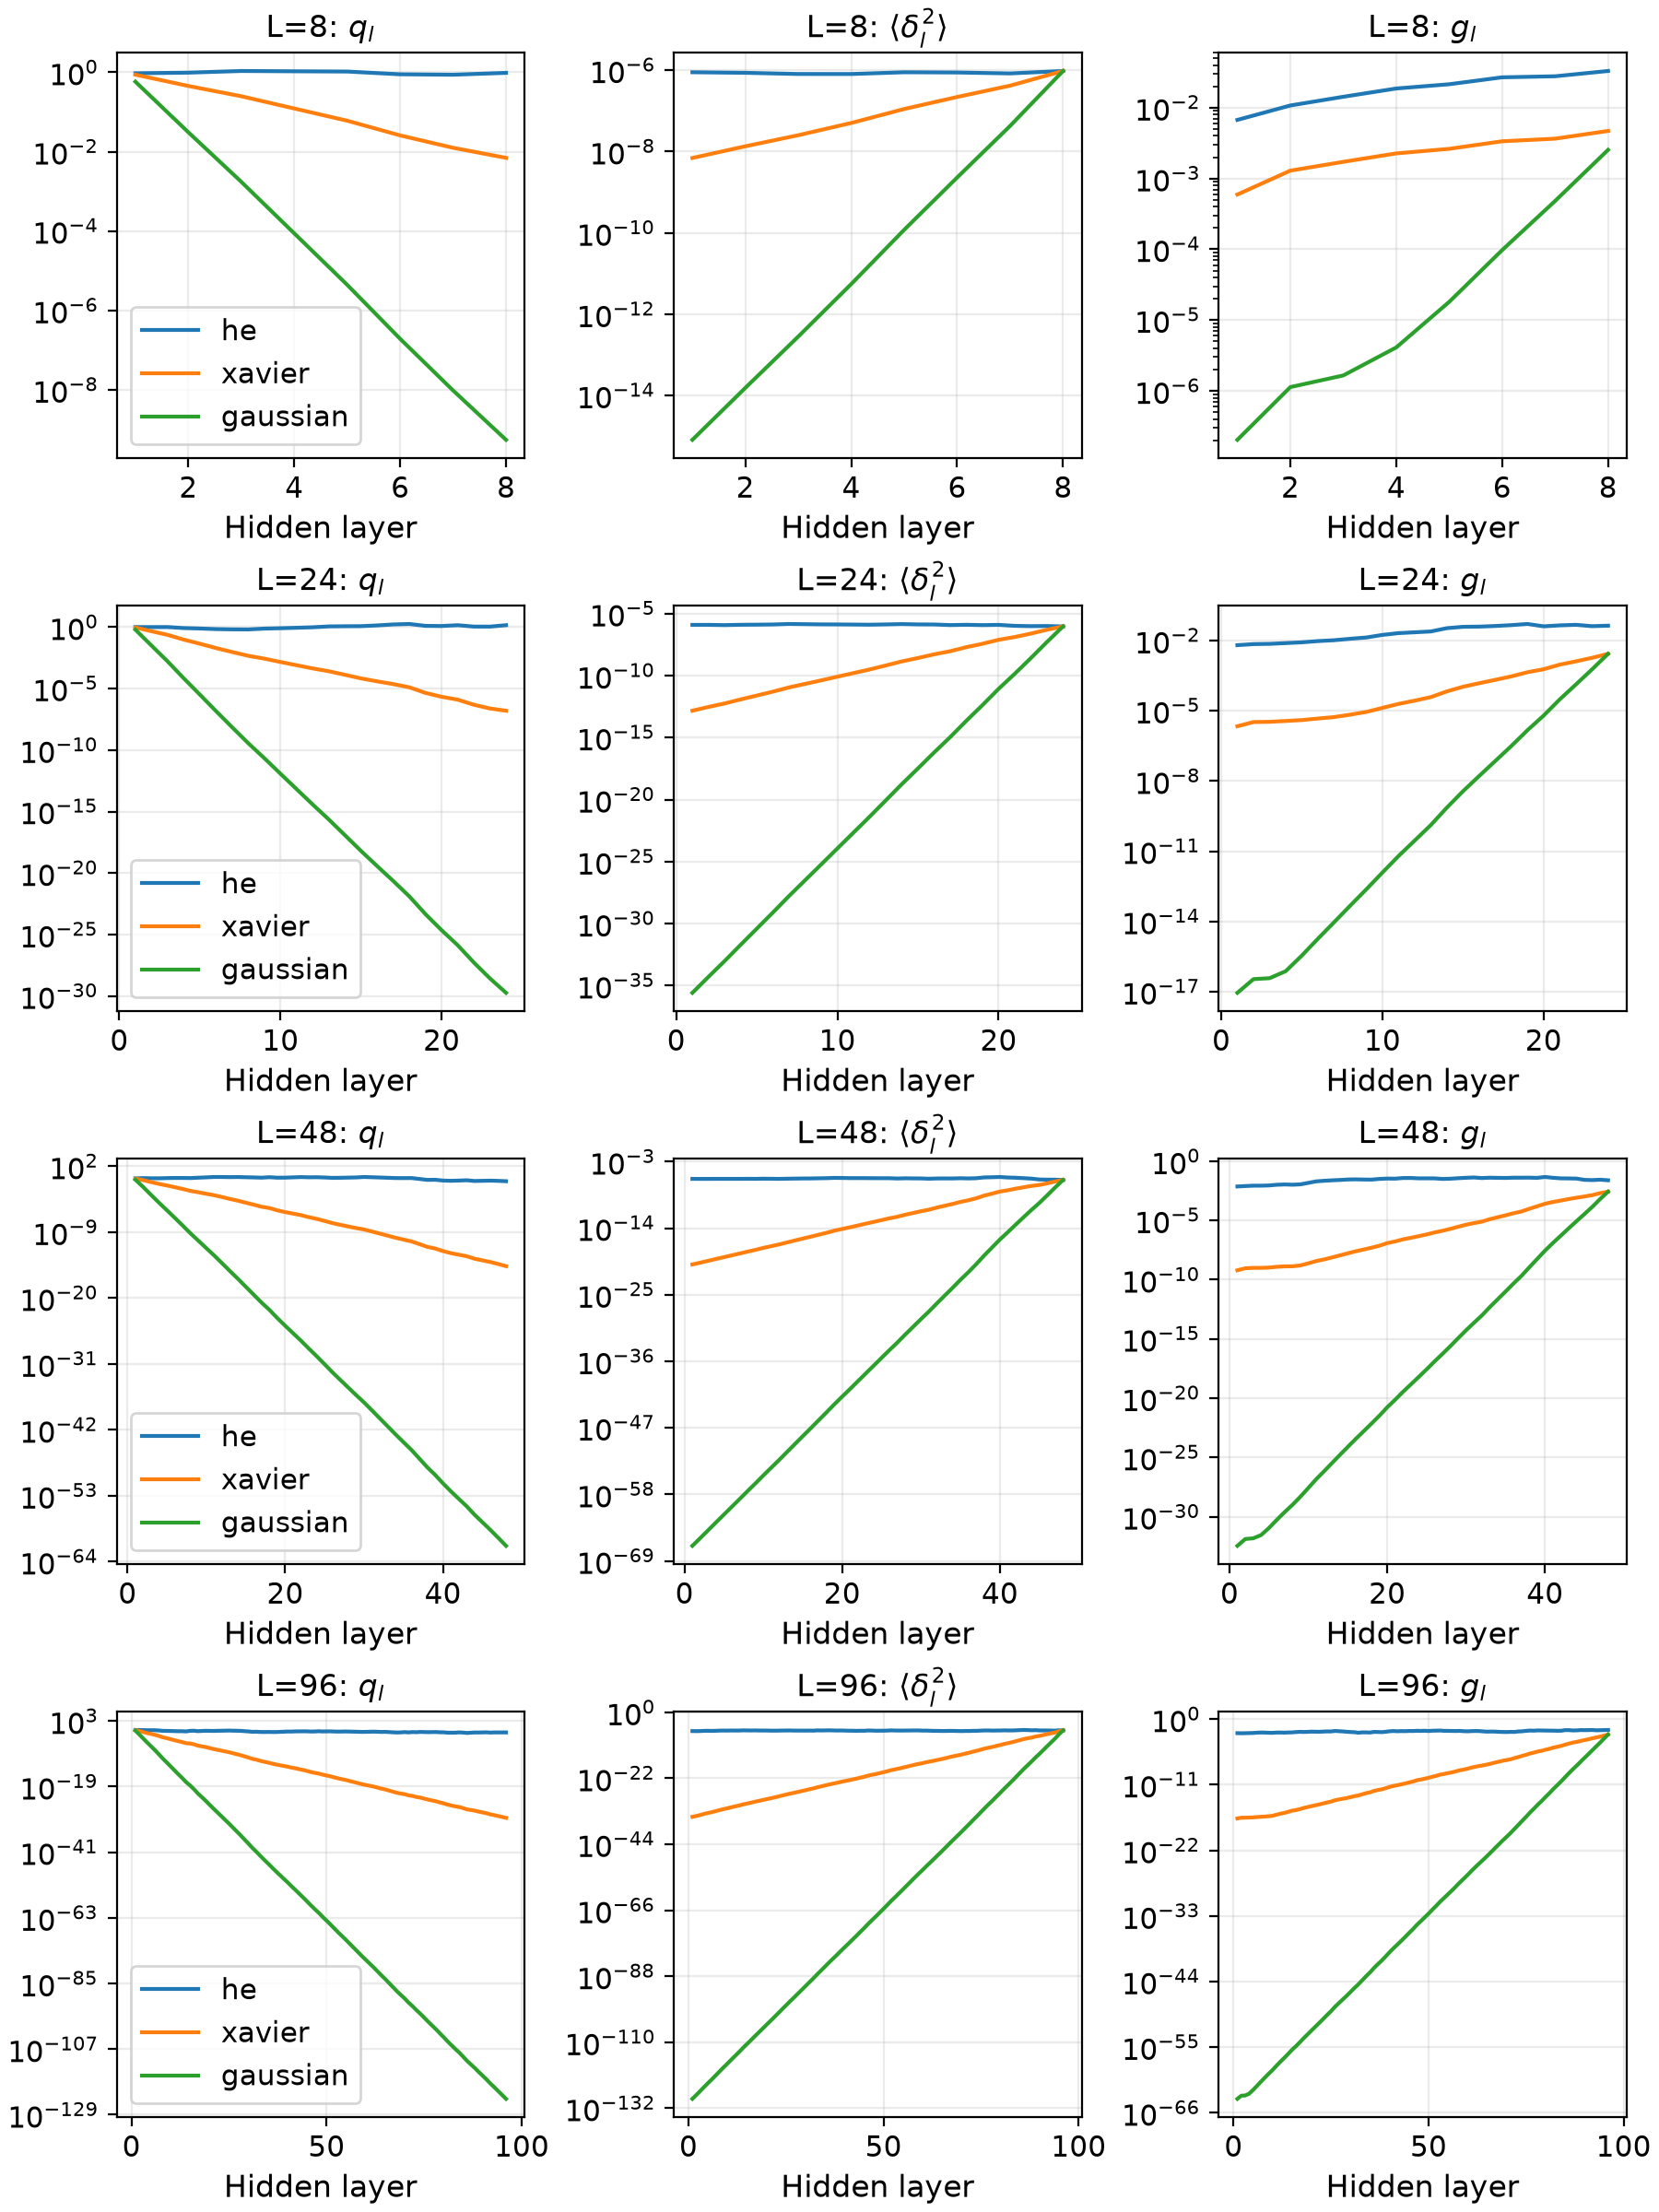
\includegraphics[width=\linewidth,height=.77\textheight,keepaspectratio]{figures/e1.png}
\caption{Сигнал, градиент по выходу и нормированный градиент параметров: все глубины и три схемы. Источники: R05, R09, R13, R06, R10, R14, R07, R11, R15, R08, R12, R16.}
\end{figure}

\clearpage

\section{E2: глубина и остаточные связи}

Заранее записанная гипотеза: He сохраняет масштаб обычной сети лишь в среднем; для остаточной сети (1.13) предсказывает $(1+\alpha^2c)^L$, $c\approx2$. При $\alpha=1$ сигнал растёт экспоненциально, а при $\alpha=L^{-1/2}$ ограничивается $e^c$. Оптимизация и конечная ширина могут нарушать независимость слагаемых.

\begin{table}[H]\centering\small\setlength{\tabcolsep}{4pt}
\caption{Обучение сетей разной глубины: все условия E2.}
\FitTable{\begin{tabular}{lrrrrrrr}
\toprule
Архитектура & L & $\rho_T$ & GI & AVD & val acc. & Статус & Источник \\
\midrule
MLP & 8 & 0.5801 & 0.739 & 0.469 & 0.4558 & OK & R22 \\
MLP & 24 & 0.6557 & 0.7856 & 0.758 & 0.4056 & OK & R23 \\
MLP & 48 & 0.7112 & 0.8132 & 1.045 & 0.3294 & OK & R24 \\
MLP & 96 & 0.8061 & 1.116 & 0.8217 & 0.2204 & OK & R25 \\
Res $\alpha=1$ & 8 & -- & 1.253 & -- & -- & сбой & R26 \\
Res $\alpha=1$ & 24 & -- & 1.279 & -- & -- & сбой & R27 \\
Res $\alpha=1$ & 48 & -- & 1.434 & -- & -- & сбой & R28 \\
Res $\alpha=1$ & 96 & -- & 1.286 & -- & -- & сбой & R29 \\
Res $\alpha=L^{-1/2}$ & 8 & 0.5184 & 1.253 & 0.4786 & 0.4688 & OK & R30 \\
Res $\alpha=L^{-1/2}$ & 24 & 0.5085 & 1.495 & 0.5452 & 0.469 & OK & R31 \\
Res $\alpha=L^{-1/2}$ & 48 & 0.5202 & 1.632 & 0.5518 & 0.477 & OK & R32 \\
Res $\alpha=L^{-1/2}$ & 96 & 0.5136 & 1.773 & 0.5427 & 0.4704 & OK & R33 \\
\bottomrule
\end{tabular}}
\end{table}

Численный сбой является наблюдаемым отрицательным результатом, а не завершёнными тремя эпохами. Для него отсутствующие итоговые метрики обозначены прочерком; не используются случайная точность или нулевая ошибка вместо отсутствующего измерения.

GI при сбое вычислен только по доступным измерениям до остановки, поэтому не сопоставляется как полноценная девятиточечная медиана с завершёнными запусками. Доли нулей в сводке сбоя относятся к исходной пробе. Точная остановка:

\begin{table}[H]\centering\small\setlength{\tabcolsep}{4pt}
\caption{Число обновлений до численного сбоя при единичной ветви.}
\FitTable{\begin{tabular}{lrrr}
\toprule
L & Завершено эпох & Шагов SGD & Источник \\
\midrule
8 & 0 & 3 & R26 \\
24 & 0 & 1 & R27 \\
48 & 0 & 1 & R28 \\
96 & 0 & 1 & R29 \\
\bottomrule
\end{tabular}}
\end{table}

Первая необучаемая глубина (rho≥0.9 либо численный сбой): MLP: не найдена в профиле; Res $\alpha=1$: 8; Res $\alpha=L^{-1/2}$: не найдена в профиле.

\begin{table}[H]\centering\small\setlength{\tabcolsep}{4pt}
\caption{Глубина и число параметров обычных и остаточных сетей.}
\FitTable{\begin{tabular}{lrrrr}
\toprule
Архитектура & L & Параметры & Линейных слоёв & Источник \\
\midrule
MLP & 8 & 1249802 & 9 & R22 \\
MLP & 96 & 7039498 & 97 & R25 \\
Res $\alpha=1$ & 8 & 1841930 & 18 & R26 \\
Res $\alpha=1$ & 96 & 13421322 & 194 & R29 \\
Res $\alpha=L^{-1/2}$ & 8 & 1841930 & 18 & R30 \\
Res $\alpha=L^{-1/2}$ & 96 & 13421322 & 194 & R33 \\
\bottomrule
\end{tabular}}
\end{table}

\begin{figure}[H]\centering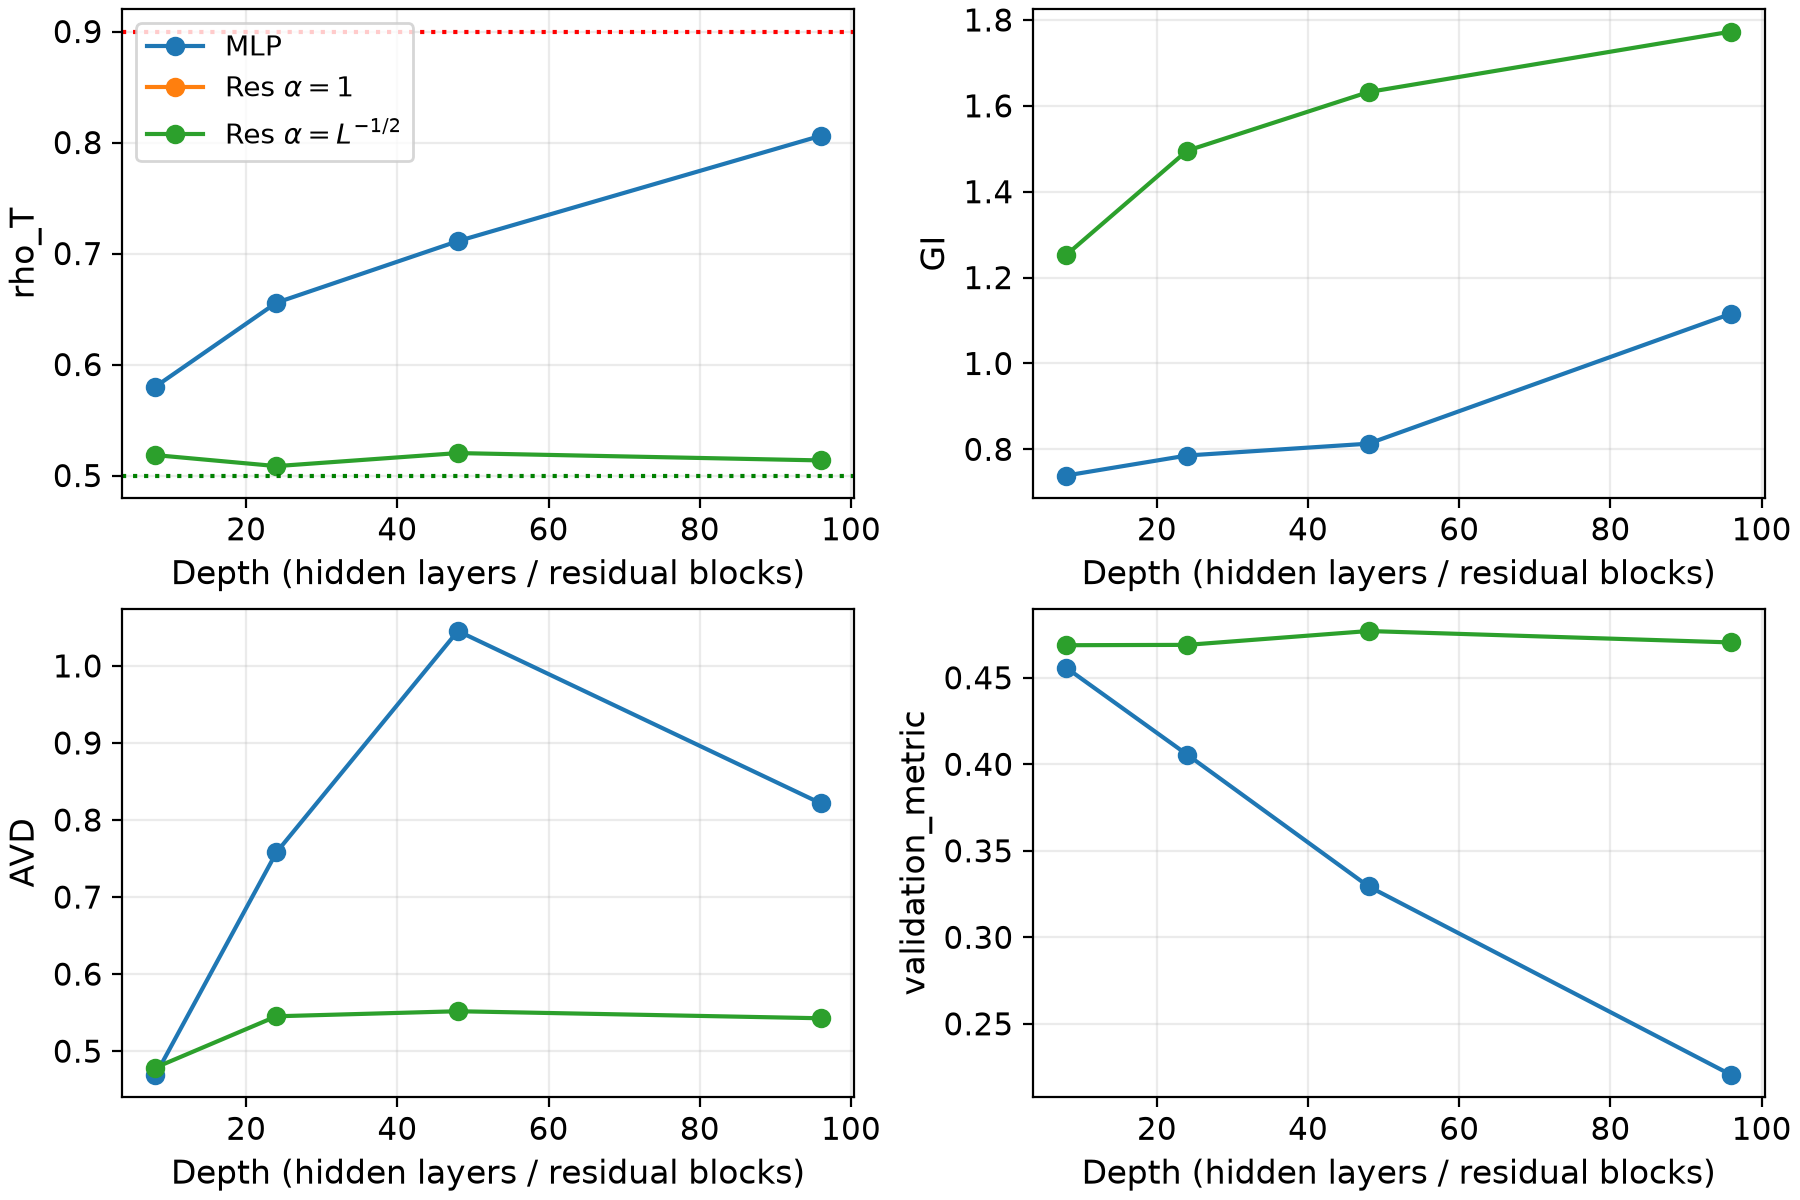
\includegraphics[width=\linewidth,height=.47\textheight,keepaspectratio]{figures/e2.png}
\caption{Результаты трёх эпох: численно неуспешные условия не выводятся как итоговые кривые. Частичные GI до сбоя сохранены в таблице. Источники соответствуют таблице E2.}
\end{figure}

Проверка роста сигнала до обучения. Для единичной ветви сравнивается корень степени L, поскольку прямое отношение накапливает малые ошибки каждого блока. Для масштабированной ветви применяется именно верхняя граница 1.2 exp(c).

\begin{table}[H]\centering\small\setlength{\tabcolsep}{4pt}
\caption{Рост сигнала остаточных сетей до обучения.}
\FitTable{\begin{tabular}{lrrrrrr}
\toprule
Ветвь & L & c & $q_L/q_0$ & $(q_L/q_0)^{1/L}$ & Порог & Источник \\
\midrule
1 & 8 & 2.134 & 6006 & 2.967 & PASS & R26 \\
1 & 24 & 1.718 & 1.855e+11 & 2.948 & PASS & R27 \\
1 & 48 & 1.833 & 3.773e+22 & 2.954 & PASS & R28 \\
1 & 96 & 1.742 & 2.861e+45 & 2.975 & PASS & R29 \\
$L^{-1/2}$ & 8 & 2.134 & 5.477 & 1.237 & PASS & R30 \\
$L^{-1/2}$ & 24 & 1.718 & 5.693 & 1.075 & PASS & R31 \\
$L^{-1/2}$ & 48 & 1.833 & 7.179 & 1.042 & PASS & R32 \\
$L^{-1/2}$ & 96 & 1.742 & 6.996 & 1.02 & FAIL & R33 \\
\bottomrule
\end{tabular}}
\end{table}

\textbf{Зарегистрированное исключение:} на L=96 масштабированная ветвь превышает границу на 2.148\%. Этот численный порог не пройден; его нельзя объявить PASS по результатам обучения или подменить другим seed.

Отдельная проба с теми же весами и batch (R40) локализует причину: c первого блока 1.742, среднее c по 96 блокам 2.029, диапазон [1.461, 2.67]. Одно измерение первого блока не является общей константой всех ветвей конечной сети.

Точное равенство для измеренных моментов: $q_{l+1}/q_l=1+\alpha^2c_l+2\alpha\kappa_l$, где $\kappa_l=\langle h_l,F_l\rangle/q_l$. Произведение этих множителей равно 6.996, непосредственно измеренное отношение 6.996. Если сохранить все разные $c_l$, но отбросить перекрёстные члены, получится 7.442. Значит, в данном запуске перекрёстные члены суммарно уменьшают рост; превышение границы связано прежде всего с использованием заниженного c первого блока вместо разных $c_l$. Предположения общего c и нулевого эмпирического перекрёстного момента не выполняются точно. Равенство с полными моментами проверено отдельным автоматическим тестом. Исходное невыполнение порога сохраняется в выводе.


\subsection*{Повторная проверка E2}
Повтор проведён после проверки реализации без изменения конфигурации: seed 987693601, SGD с momentum 0.9, learning rate 0.003, batch 128, три эпохи, ширина 256, исходный split и все двенадцать условий. Первоначальные запуски сохранены; повтор имеет отдельные RUN\_ID. Проверены инициализация обоих слоёв ветви, нулевые bias, масштаб $L^{-1/2}$, hook измерения $q$ и определение $c$ по первой ветви. Ошибка реализации не обнаружена.
\begin{table}[H]\centering\footnotesize
\setlength{\tabcolsep}{4pt}
\caption{Повтор E2: исходные seed, данные и гиперпараметры; сбои не заменены успешными запусками.}\label{tab:repeat_e2}
\begin{tabular}{lrrrrll}
\toprule
Архитектура & L & Шаги & $\rho_T$ & Val acc. & Статус & Ист. \\
\midrule
Plain & 8 & 1008 & 0.580099 & 0.455800 & завершён & S1 \\
Plain & 24 & 1008 & 0.655689 & 0.405600 & завершён & S2 \\
Plain & 48 & 1008 & 0.711155 & 0.329400 & завершён & S3 \\
Plain & 96 & 1008 & 0.806055 & 0.220400 & завершён & S4 \\
Res. $\alpha=1$ & 8 & 3 & --- & --- & сбой & S5 \\
Res. $\alpha=1$ & 24 & 1 & --- & --- & сбой & S6 \\
Res. $\alpha=1$ & 48 & 1 & --- & --- & сбой & S7 \\
Res. $\alpha=1$ & 96 & 1 & --- & --- & сбой & S8 \\
Res. $\alpha=L^{-1/2}$ & 8 & 1008 & 0.518377 & 0.468800 & завершён & S9 \\
Res. $\alpha=L^{-1/2}$ & 24 & 1008 & 0.508478 & 0.469000 & завершён & S10 \\
Res. $\alpha=L^{-1/2}$ & 48 & 1008 & 0.520223 & 0.477000 & завершён & S11 \\
Res. $\alpha=L^{-1/2}$ & 96 & 1008 & 0.513602 & 0.470400 & завершён & S12 \\
\bottomrule
\end{tabular}
\end{table}


\begin{table}[H]\centering\small
\setlength{\tabcolsep}{4pt}
\caption{Повторная проверка границы роста масштабированной остаточной сети.}\label{tab:repeat_growth}
\begin{tabular}{rrrrl}
\toprule
L & $c_1$ & $q_L/q_0$ & $1.2e^{c_1}$ & Порог \\
\midrule
8 & 2.133690 & 5.477458 & 10.135174 & PASS \\
24 & 1.717932 & 5.693482 & 6.687589 & PASS \\
48 & 1.832620 & 7.179433 & 7.500292 & PASS \\
96 & 1.741828 & 6.996440 & 6.849322 & FAIL \\
\bottomrule
\end{tabular}
\end{table}


Начальные вторые моменты повторяют исходные значения с относительной ошибкой менее $10^{-12}$. В частности, при L=96 снова получено $q_L/q_0=6.996440$ при границе 6.849322. Исходный FAIL воспроизведён, а не устранён сменой seed или порога.

Для конечной ширины точное равенство содержит перекрёстный момент:
\begin{equation}
\frac{q_l}{q_{l-1}}=1+\alpha^2 c_l+2\alpha r_l,\quad
r_l=\frac{\mathbb E[h_{l-1}F_l(h_{l-1})]}{q_{l-1}}.
\end{equation}
Произведение этих измеренных множителей совпадает с $q_L/q_0$ с относительной ошибкой менее $10^{-12}$. Замена всех $c_l$ первым $c_1$ и отбрасывание $r_l$ дают приближение среднего поля, а не тождество отдельной конечной сети. Поэтому воспроизведение подтверждает численную причину отклонения; оно не превращает невыполненный порог в PASS. Основной трёхseedовый E3 и его исходная гипотеза не менялись.

\section{Карта обучаемости}

\begin{figure}[H]\centering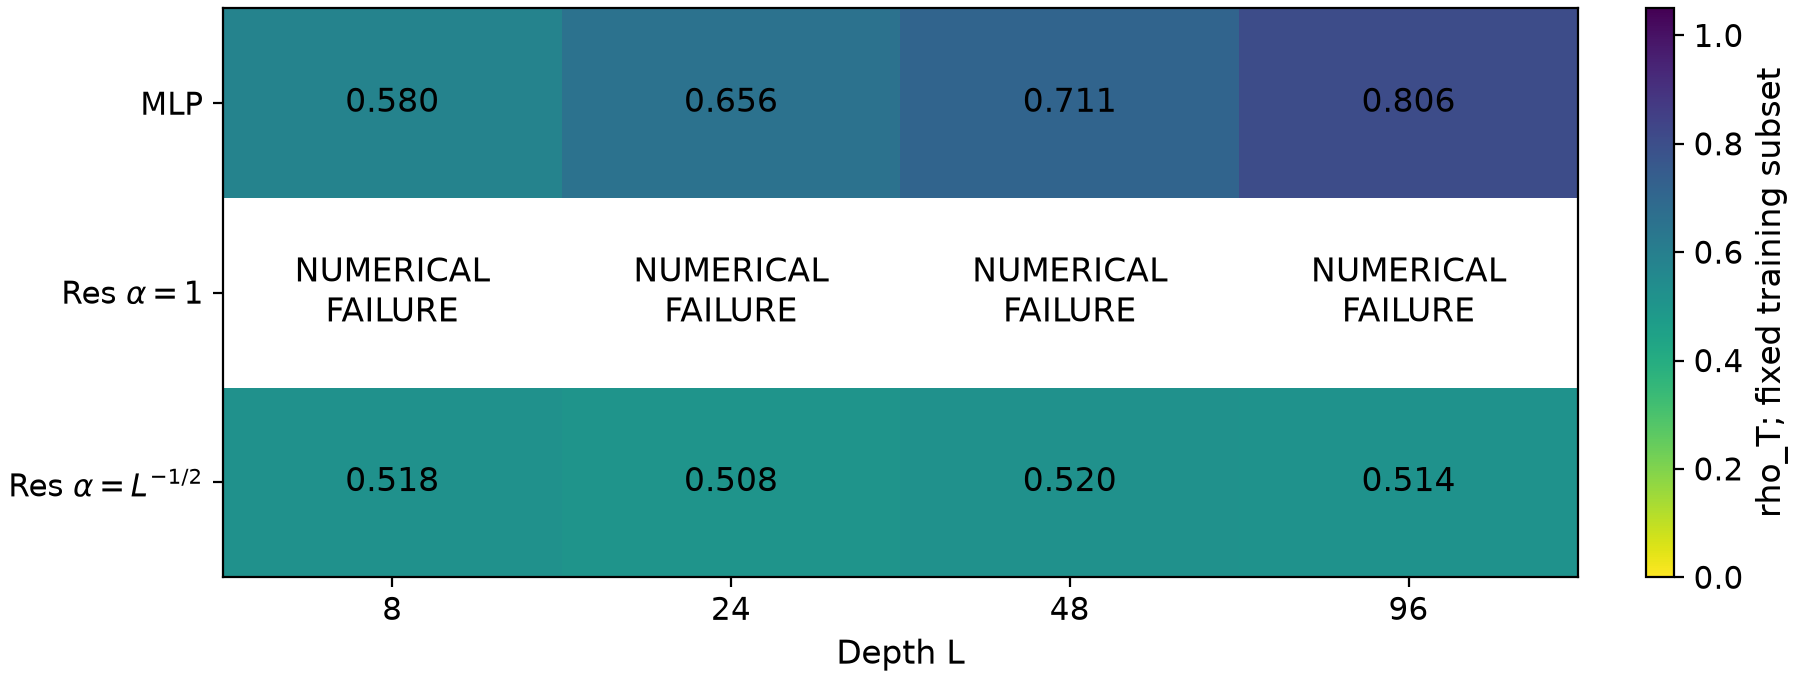
\includegraphics[width=\linewidth,height=.35\textheight,keepaspectratio]{figures/map.png}
\caption{Двумерный срез: глубина $\times$ архитектура $\to\rho_T$. Численный сбой показан текстом, а не искусственным значением.}
\end{figure}

Изменяются только глубина и архитектура; фиксированы: CIFAR-10 и его разбиение, полный train, нормализация данных, seed профиля, ширина 256, He, ReLU, отсутствие нормализации слоёв, SGD momentum 0.9, LR=0.003, batch 128, три эпохи, float32, отсутствие AMP и клиппинга, подмножество вычисления rho и расписание измерений. Источники ячеек: таблица E2 и реестр RUN\_ID.

Порог $\rho_T\le0.5$ обозначает обучаемость; $\rho_T\ge0.9$ -- необучаемость; промежуточные значения -- пограничный режим. Более высокая val accuracy сама по себе не означает выполнения порога обучаемости. Карта относится к одному seed и одному разбиению и не доказывает универсальную границу глубины.

\section{E3: основное парное сравнение}

До обучения E3 сформулирована гипотеза о меньшей относительной ошибке остаточной сети. A: обычная MLP, 96 скрытых слоёв. B: остаточная MLP, 96 блоков, alpha=1/sqrt(96). Единственный изменяемый фактор: архитектура (model.name); остальные поля модели одинаковы.

Основная метрика: $\rho_T$, меньше лучше. Ожидается положительная разность A−B. Условие опровержения: отсутствие трёх положительных разностей либо средняя разность меньше двух выборочных стандартных отклонений. Все остальные условия совпадают, включая буквальные seeds 1, 2, 3.

\begin{table}[H]\centering\small\setlength{\tabcolsep}{4pt}
\caption{Основное сравнение E3: все три парных seed.}
\FitTable{\begin{tabular}{lrrrr}
\toprule
seed & $\rho_T(A)$ & $\rho_T(B)$ & $\Delta_s$ & A / B \\
\midrule
1 & 0.8074 & 0.5239 & 0.2835 & R41 / R44 \\
2 & 0.8038 & 0.5162 & 0.2877 & R42 / R45 \\
3 & 0.8003 & 0.4977 & 0.3026 & R43 / R46 \\
\bottomrule
\end{tabular}}
\end{table}

Средняя разность 0.2913, выборочное sΔ=0.01003, 2sΔ=0.02007. По установленному правилу: различие установлено. Это проверка главного эффекта на данном разбиении; три seeds отражают только случайность обучения, а не перенос на другие данные.

\begin{table}[H]\centering\small\setlength{\tabcolsep}{4pt}
\caption{Средние значения и выборочные SD в E3.}
\FitTable{\begin{tabular}{lrrrr}
\toprule
Вариант & Среднее rho & SD rho & Среднее val acc. & SD val acc. \\
\midrule
A & 0.8039 & 0.003548 & 0.2341 & 0.009979 \\
B & 0.5126 & 0.01345 & 0.4675 & 0.008649 \\
\bottomrule
\end{tabular}}
\end{table}

\section{Ответы на контрфактические вопросы}

\subsection*{1. Экстраполяция He до глубины 256}

Из R08: $\hat\chi_f=0.9804$. Формальная экстраполяция даёт $q_{256}/q_1=\hat\chi_f^{255}=0.006359$. Это прогноз по (1.4), а не измерение L=256. Даже небольшое отклонение множителя от единицы накапливается экспоненциально. Стабильность на L=16 не гарантирует ни сохранения масштаба, ни оптимизации на L=256: конечная ширина создаёт корреляции активаций и производных; при обратном проходе предположение независимости градиента от тех же весов уже приближённо. После первого обновления нарушается и предположение исходных независимых весов. Скалярный второй момент не контролирует весь спектр Якобиана.

\subsection*{2. Увеличение ширины в четыре раза}

При n=1024 и прежнем $\sigma=0.02$ прогноз $\chi=1024\sigma^2/2=0.2048$. Отдельная проба R38 дала forward 0.208, backward 0.2056, эффективных слоёв 44. Рост ширины изменяет множитель, но не делает его единичным; sigma не перенастраивалась.

\subsection*{3. Градиент по выходу и градиент по весу}

Источник R14: средние квадраты delta на первом и последнем скрытых слоях 2.604e-36 и 9.537e-07; g первого и последнего скрытых слоёв 9.064e-18 и 0.002694.

Для весов $\nabla_{W_l}L$ содержит произведение входа $h_{l-1}$ и обратного сигнала с маской ReLU. По (1.4), (1.8) уменьшение прямого сигнала при продвижении к выходу компенсируется ростом delta в том же направлении; поэтому весовые градиенты внутренних слоёв имеют близкий порядок. Первый слой имеет другую ширину входа и статистику. Однако в обязательном $g_l$ здесь учтены также bias: $\nabla_bL$ не умножается на малый вход. Поэтому полное g может существенно расти к выходу, и буквально одинаковые значения на исходном графике не заявляются. Этот предел подсказки PDF и отличие bias от весов проверены отдельным разложением R39. Константа epsilon в GI дополнительно маскирует различия величин намного меньше $10^{-12}$; такой GI не означает сохранения абсолютных градиентов.

В пробе R39 внутренние весовые $g$ (слои 2--24) лежат от $3.479\cdot10^{-17}$ до $2.521\cdot10^{-16}$, отношение максимума к минимуму равно 7.244. Для bias диапазон составляет от $4.91\cdot10^{-17}$ до 0.04318. Это измеренное разложение, а не изменение определения обязательного GI.

\begin{figure}[H]\centering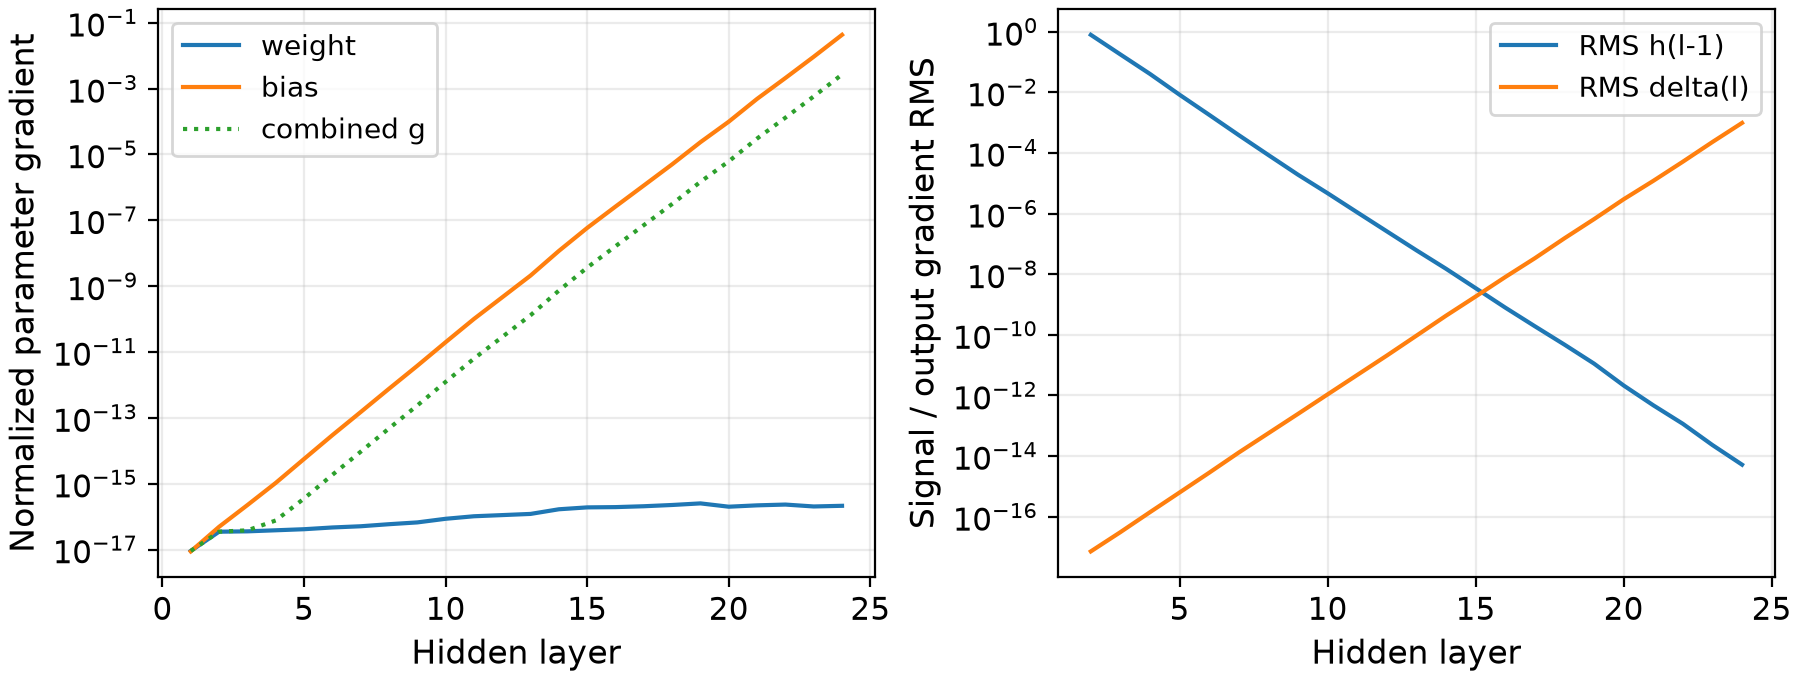
\includegraphics[width=\linewidth,height=.32\textheight,keepaspectratio]{figures/cf3.png}
\caption{Разложение весов и bias; компенсация масштабов прямого и обратного сигналов. Источник R39.}
\end{figure}

\subsection*{4. Почему единичный skip не предотвращает взрыв}

\begin{table}[H]\centering\small\setlength{\tabcolsep}{4pt}
\caption{Измеренный и предсказанный рост при единичной ветви.}
\FitTable{\begin{tabular}{lrrrr}
\toprule
L & Измерено q ratio & Прогноз $(1+c)^L$ & Ошибка корня & Источник \\
\midrule
8 & 6006 & 9299 & 0.05319 & R26 \\
24 & 1.855e+11 & 2.641e+10 & 0.08461 & R27 \\
48 & 3.773e+22 & 5.07e+21 & 0.0427 & R28 \\
96 & 2.861e+45 & 1.127e+42 & 0.08509 & R29 \\
\bottomrule
\end{tabular}}
\end{table}

Единичный член Якобиана обеспечивает прямой путь, но не убирает вклад ветви. При $\alpha=1$ накопление энергии ветвей экспоненциально; огромные логиты и производные делают обучение неустойчивым. Формула предсказывает средний рост при инициализации, а не устойчивость конечного шага SGD. Расхождения полных отношений при глубине 96 могут быть большими даже при допустимой ошибке среднего множителя за блок.

\subsection*{5. Близкая точность не означает одинаковую устойчивость}

Пара выбрана исследовательски из E2: разность val accuracy не более0.02, разность GI не менее0.5; следующая глубина для каждой конфигурации уже содержится в сетке E2, поэтому это проверка на имеющихся данных, а не независимый прогноз. Текущие конфигурации: R22 и R30; проверка следующей глубины: R23, R31. Обе исходные сети имеют глубину 8; следующий уровень профиля равен 24.

\begin{table}[H]\centering\small\setlength{\tabcolsep}{4pt}
\caption{Проверка следующей глубины для конфигураций с близкой точностью.}
\FitTable{\begin{tabular}{lrrrrr}
\toprule
Архитектура & L & val acc. & GI & $\rho_T$ & Источник \\
\midrule
MLP & 8 & 0.4558 & 0.739 & 0.5801 & R22 \\
Res $\alpha=L^{-1/2}$ & 8 & 0.4688 & 1.253 & 0.5184 & R30 \\
MLP & 24 & 0.4056 & 0.7856 & 0.6557 & R23 \\
Res $\alpha=L^{-1/2}$ & 24 & 0.469 & 1.495 & 0.5085 & R31 \\
\bottomrule
\end{tabular}}
\end{table}

При переходе от глубины 8 к 24 accuracy обычной сети снизилась на 0.0502, а $\rho_T$ выросла на 0.07559 (R22/R23). Для масштабированной остаточной сети accuracy изменилась на +0.0002, а $\rho_T$ --- на $-0.009899$ (R30/R31). Одинаково устойчивыми эти конфигурации считать нельзя. В выбранной паре масштабированная остаточная сеть сохраняет точность лучше, хотя её GI выше: GI не является достаточным сертификатом устойчивости при сравнении разных архитектур, масштаба ветви и нормировки числа параметров. Проверка соседней глубины не даёт права объявить общий причинный закон по четырём точкам.


\subsection*{Заключение}
He сохраняет средний масштаб сигнала значительно лучше Xavier и Gaussian с фиксированным малым $\sigma$. Масштабирование остаточной ветви предотвращает наблюдавшиеся численные сбои единичной ветви и снижает $\rho_T$ на глубине 96: средняя парная разность равна 0.291256 при SD 0.010034. По правилу задания различие установлено. Однако граница роста $1.2e^c$ в одном условии не выполнена, а значения $\rho_T$ большей части обученных сетей остаются пограничными. Вывод относится к одному split, трём эпохам и выбранным архитектурам; разные числа параметров plain/residual следует учитывать при переносе сравнения.
\clearpage
\renewcommand{\refname}{Список использованных источников}
\begin{thebibliography}{9}
\addcontentsline{toc}{section}{Список использованных источников}
\bibitem{teacher} Лабораторная работа 1. Почему глубокая сеть обучается или не обучается. Инициализация, нормализация и остаточные связи. Курс «Нейронные сети». Методические указания, 2026.
\end{thebibliography}
\clearpage
\section*{Приложение. Идентификация запусков}
\addcontentsline{toc}{section}{Приложение. Идентификация запусков}
\begingroup\small\setstretch{1.05}
\begin{longtable}{@{}l>{\raggedright\arraybackslash}p{3.5cm}p{10.8cm}@{}}
\caption{Полные RUN\_ID источников результатов.}\\
\toprule Код & Условие & RUN\_ID \\ \midrule \endhead
\hypertarget{R03}{R03} & budget deep mlp8 & {\fontsize{8.8}{11}\selectfont\texttt{f35bc17d724ab6701081-82b8437770094d618463160db216475b}} \\
\hypertarget{R04}{R04} & budget residual mlp96 & {\fontsize{8.8}{11}\selectfont\texttt{7985b20739cc3e05fbf7-3ee53f04473f463e91f20cf0a9489de8}} \\
\hypertarget{R05}{R05} & E1 he 8 & {\fontsize{8.8}{11}\selectfont\texttt{835b5aa0a6f48bd5d01a-f54918af472940a8bda1544bbb329a16}} \\
\hypertarget{R06}{R06} & E1 he 24 & {\fontsize{8.8}{11}\selectfont\texttt{daa1a446d8bceaabc44b-0020695fecef4a11b1175d6777f6a866}} \\
\hypertarget{R07}{R07} & E1 he 48 & {\fontsize{8.8}{11}\selectfont\texttt{534625583d5990da50fd-6b7164b3c8a84bf484d39fb270e6e418}} \\
\hypertarget{R08}{R08} & E1 he 96 & {\fontsize{8.8}{11}\selectfont\texttt{42b49b40517988afe273-40a880f74e9442d594137504c5cea87a}} \\
\hypertarget{R09}{R09} & E1 xavier 8 & {\fontsize{8.8}{11}\selectfont\texttt{49b8b7c74a10aa5a1a64-72e0590df7f948ef842011c216d05444}} \\
\hypertarget{R10}{R10} & E1 xavier 24 & {\fontsize{8.8}{11}\selectfont\texttt{6144c2152d8b81e8e800-e50fafcc7ae24bbc85d0ee8a28e452df}} \\
\hypertarget{R11}{R11} & E1 xavier 48 & {\fontsize{8.8}{11}\selectfont\texttt{67cc401b4bb5ac8738d7-601c39a72896441bb8dc2572ef47ddb1}} \\
\hypertarget{R12}{R12} & E1 xavier 96 & {\fontsize{8.8}{11}\selectfont\texttt{e6a6b92aec9f1b597e47-59437c84059143c0a7a006c5e2cc9afa}} \\
\hypertarget{R13}{R13} & E1 gaussian 8 & {\fontsize{8.8}{11}\selectfont\texttt{d268af8bc42f48f6aedb-28e24e9853d241b4964e0fcc831a33d0}} \\
\hypertarget{R14}{R14} & E1 gaussian 24 & {\fontsize{8.8}{11}\selectfont\texttt{4e0cd7079a80871a0fd2-0bd00f5a2a5c4d44b609ad1887b3c9ae}} \\
\hypertarget{R15}{R15} & E1 gaussian 48 & {\fontsize{8.8}{11}\selectfont\texttt{1b3500a435561a91443f-289aa271826f4edeab053939b401b384}} \\
\hypertarget{R16}{R16} & E1 gaussian 96 & {\fontsize{8.8}{11}\selectfont\texttt{25e23c0eead538f90a0d-589b8c19d95b4d7d99ce737c9178879a}} \\
\hypertarget{R17}{R17} & LR 0.001 & {\fontsize{8.8}{11}\selectfont\texttt{a33e03472d5d93fa15fc-c04ce6a1e9de4cbc9a55963b7c6efe8f}} \\
\hypertarget{R18}{R18} & LR 0.003 & {\fontsize{8.8}{11}\selectfont\texttt{2a04c5f5545b92efa370-90029285e78c4036b5045079e0040cb3}} \\
\hypertarget{R19}{R19} & LR 0.01 & {\fontsize{8.8}{11}\selectfont\texttt{400ffa75051d3a2de91e-33949168d69e4583b9df2dcaec27996f}} \\
\hypertarget{R20}{R20} & LR 0.03 & {\fontsize{8.8}{11}\selectfont\texttt{1d8d7a73e2b3bb3c5592-5d490d650a6b489f9f3cd00163c0e9e8}} \\
\hypertarget{R21}{R21} & LR 0.1 & {\fontsize{8.8}{11}\selectfont\texttt{8f701c927e6893a8a94d-d190e54bf6b140c1b06756b2fe7e9f69}} \\
\hypertarget{R22}{R22} & E2 plain 8 & {\fontsize{8.8}{11}\selectfont\texttt{072042389309a9d0e7ed-1f2cf56abb4346aaaf4c984d8453e7cb}} \\
\hypertarget{R23}{R23} & E2 plain 24 & {\fontsize{8.8}{11}\selectfont\texttt{58dafff69939ce9dbcb6-e66dade201944d788880ac3ce569c948}} \\
\hypertarget{R24}{R24} & E2 plain 48 & {\fontsize{8.8}{11}\selectfont\texttt{6ed9fd9deccbf25d4dbe-cc78467e46a3445c94defd782f4fc343}} \\
\hypertarget{R25}{R25} & E2 plain 96 & {\fontsize{8.8}{11}\selectfont\texttt{f02840c34662292f2550-7cdcbabd38c5472aa0d47e49f5bb04a5}} \\
\hypertarget{R26}{R26} & E2 residual unit 8 & {\fontsize{8.8}{11}\selectfont\texttt{f6f40777a94fe870b3f5-7aca80a890724e3f9bda60579352ab21}} \\
\hypertarget{R27}{R27} & E2 residual unit 24 & {\fontsize{8.8}{11}\selectfont\texttt{760974ee261830470993-0f7a8c6bd49543a3841314e919684f77}} \\
\hypertarget{R28}{R28} & E2 residual unit 48 & {\fontsize{8.8}{11}\selectfont\texttt{3dbe3c0827c108c86e2a-e047f8229707429c93184bc75d3c244e}} \\
\hypertarget{R29}{R29} & E2 residual unit 96 & {\fontsize{8.8}{11}\selectfont\texttt{bc1cfc0f52214e75038c-38c277eeab774b1194dd1844f372dc67}} \\
\hypertarget{R30}{R30} & E2 residual scaled 8 & {\fontsize{8.8}{11}\selectfont\texttt{43ffb961514ceb1ea9d8-f27c2da7032640ada2cfd54df8a038c8}} \\
\hypertarget{R31}{R31} & E2 residual scaled 24 & {\fontsize{8.8}{11}\selectfont\texttt{b48bb6d07e183f729073-5be4e5eaf78049d6964cdcc1cb02e95c}} \\
\hypertarget{R32}{R32} & E2 residual scaled 48 & {\fontsize{8.8}{11}\selectfont\texttt{1ef26c51c6f46c53cce1-8d3592e5eea64c9eaf0fe094da598ca9}} \\
\hypertarget{R33}{R33} & E2 residual scaled 96 & {\fontsize{8.8}{11}\selectfont\texttt{0f7c5a6ad6fc18622306-27adbadc93c941d1af43fd88e9bac108}} \\
\hypertarget{R34}{R34} & E1 after epoch gaussian 8 & {\fontsize{8.8}{11}\selectfont\texttt{f65cc36c6722183555aa-55a880a1f0d6428a854d9626cdcb4442}} \\
\hypertarget{R35}{R35} & E1 after epoch gaussian 24 & {\fontsize{8.8}{11}\selectfont\texttt{6a2dbdc4016e278bf3ac-57c9588a9af74ea1b49fabff4156f78a}} \\
\hypertarget{R36}{R36} & E1 after epoch gaussian 48 & {\fontsize{8.8}{11}\selectfont\texttt{46cc2d0333f98ec911be-63cd8333272b4ec09520e3337f7b87cf}} \\
\hypertarget{R37}{R37} & E1 after epoch gaussian 96 & {\fontsize{8.8}{11}\selectfont\texttt{670167bc6a9b50380a01-fe8eb710b34741b4a0978cfb2c3294a7}} \\
\hypertarget{R38}{R38} & CF2 gaussian width1024 depth96 & {\fontsize{8.8}{11}\selectfont\texttt{e5d33ffe2c320c0cf4ed-90f1f3c566024a2684f150ddc75997b6}} \\
\hypertarget{R39}{R39} & CF3 weight bias decomposition & {\fontsize{8.8}{11}\selectfont\texttt{7cef8aaa61602a4f04d9-91b54d0671914614a3854f8c4544cee4}} \\
\hypertarget{R40}{R40} & E2 scaled96 growth diagnosis & {\fontsize{8.8}{11}\selectfont\texttt{3d2329355cfed30d7490-9c4f04a2bdf744f3a1b3c4df418355b6}} \\
\hypertarget{R41}{R41} & E3 A seed1 & {\fontsize{8.8}{11}\selectfont\texttt{e8c645d9482cd256deae-3f76ac4a3a8949d1af2fd196756c229b}} \\
\hypertarget{R42}{R42} & E3 A seed2 & {\fontsize{8.8}{11}\selectfont\texttt{3306f27ee19bbcebd235-ffc3d19080444f2e86a38406c6784fb8}} \\
\hypertarget{R43}{R43} & E3 A seed3 & {\fontsize{8.8}{11}\selectfont\texttt{3a67488efc107b654691-80b220070f3146d985a3ab8ca3068b80}} \\
\hypertarget{R44}{R44} & E3 B seed1 & {\fontsize{8.8}{11}\selectfont\texttt{779d5c921f74c67065a7-644d33a4885e46dc89cb2d71aa80648d}} \\
\hypertarget{R45}{R45} & E3 B seed2 & {\fontsize{8.8}{11}\selectfont\texttt{0433af61b3f2e9d2763d-399fdc59a4944ec58dcf970657b2a013}} \\
\hypertarget{R46}{R46} & E3 B seed3 & {\fontsize{8.8}{11}\selectfont\texttt{dc6ad98cb134159efb9f-a47999757e4141b29594336febc1a142}} \\
\hypertarget{S1}{S1} & E2 repeat plain 8 & {\fontsize{8.8}{11}\selectfont\texttt{65e1a337699f7d318a80-201fe612c4a84a42a19926ea3d7782a4}} \\
\hypertarget{S2}{S2} & E2 repeat plain 24 & {\fontsize{8.8}{11}\selectfont\texttt{58c4a5b0fbd2cb61eeb0-f738cdd7db9d4b92bf70db8ac8ea249a}} \\
\hypertarget{S3}{S3} & E2 repeat plain 48 & {\fontsize{8.8}{11}\selectfont\texttt{6518619604d0be0f725c-83be1e71337d4dacb3df334b53e45a8a}} \\
\hypertarget{S4}{S4} & E2 repeat plain 96 & {\fontsize{8.8}{11}\selectfont\texttt{0ad4db95ba5351f181f1-d74e3e294ac343639ded726f44455466}} \\
\hypertarget{S5}{S5} & E2 repeat residual unit 8 & {\fontsize{8.8}{11}\selectfont\texttt{bf177927e88a116f4fa2-913dea3136574bd4ad1d0eee72b147af}} \\
\hypertarget{S6}{S6} & E2 repeat residual unit 24 & {\fontsize{8.8}{11}\selectfont\texttt{9ef4e5810a0ee78b86dc-1ac124de9ef44f2ebf0e6f8cf63afc83}} \\
\hypertarget{S7}{S7} & E2 repeat residual unit 48 & {\fontsize{8.8}{11}\selectfont\texttt{36c78e3aaaf99af7fab1-0b888b0572ac4376827d3d557534cc75}} \\
\hypertarget{S8}{S8} & E2 repeat residual unit 96 & {\fontsize{8.8}{11}\selectfont\texttt{9e681ade28ea46592003-91b3c5be62ac46babb763569a5a5c6c7}} \\
\hypertarget{S9}{S9} & E2 repeat residual scaled 8 & {\fontsize{8.8}{11}\selectfont\texttt{e61bf57c3fd3816e03cb-3e7d0d38cd52461b9ab73bbd1d7b096e}} \\
\hypertarget{S10}{S10} & E2 repeat residual scaled 24 & {\fontsize{8.8}{11}\selectfont\texttt{29b49364d2ebfef77faf-c435d806fe6a4b46930dd15e53540c4a}} \\
\hypertarget{S11}{S11} & E2 repeat residual scaled 48 & {\fontsize{8.8}{11}\selectfont\texttt{ce434c0816f5ed4ab494-77a0d1b4f5004ef9813d4bde491bed61}} \\
\hypertarget{S12}{S12} & E2 repeat residual scaled 96 & {\fontsize{8.8}{11}\selectfont\texttt{ac53b3d6d7866c853cfc-b8b2a6ca288146a48a2576b0c4611b19}} \\
\bottomrule\end{longtable}\endgroup
